\documentclass[english]{article}
\usepackage[T1]{fontenc}
\usepackage[utf8]{inputenc}
\usepackage{graphicx}

\usepackage{float}
\usepackage{babel}

\usepackage{array}
\usepackage{multirow}

\usepackage[font=small,labelfont=bf,labelsep=space]{caption}
\captionsetup{
  figurename = Figure,
  tablename = Table
}

\makeatletter

\providecommand{\tabularnewline}{\\}

\makeatother

\begin{document}

\title{
    Proyecto Final para la obtención del título: Ingeniero en Informática
    \tabularnewline
    \large Future Virtual Particle Method for Pedestrian Navigation
}

\author{
  Castiglione, Gonzalo\\
  \texttt{gcastigl@gmail.com}
  \and
  Marseillan, Agustin\\
  \texttt{agustinmarseillan@gmail.com}
  \and
  Dr. Parisi, Daniel Ricardo \\
  \texttt{dparisi@itba.edu.ar}
}
\date{}

\maketitle

\vspace{8cm}
\begin{center}
    
\includegraphics[scale=0.1]{pics/ITBA}
    \par
\end{center}

\pagebreak{}

\tableofcontents{}

\pagebreak{}

\begin{abstract}
% Pedestrians are modeled as objects affected by repulsive and attractive forces in the Social Force Model (SFM). 
This paper presents an avoidance collision method based in pedestrian self
governed decisions, by calculating the position of every pedestrian
in the future, a given pedestrian can adjust his velocity vector to
avoid collisions instead of being affected by a repulsive force. \\
The model was tested using three different scenarios and compared 
against the Social Force Model obtaining more natural navigation,
reduced number of collisions, increased average
speed and reduced average deviation angle of navigating pedestrians.
\textbf{keywords:} pedestrian, collision avoidance, future virtual
particle, force model.
\end{abstract}

\section{Introduction}
    
    \subsection{Motivation and previous work}
    
    Navigation of biological, synthetic or virtual agents is a relevant
    problem in several fields such as pedestrian dynamics, moving robots
    and animation of characters for video games and motion pictures.
    
    Modelling and simulating the displacement of agents through arbitrarily
    complex environments may be stated in an hierarchical structure of
    mechanisms depending mainly on the distance from the agent. This level
    has been named, from closer to further, as operational (walking, lowest
    level physical-computational model for displacement), tactical (way-finding,
    route choice) and strategic (general activity planning) \cite{key-hoog2004}.
    These levels are not independent, factors affecting one level may
    impact in the following and vice-versa, for example, the route choice
    may vary due to congestion of agents produced from previous route
    choice and walking behavior. Also, obstacles can impact on the operational
    level or tactical level depending on the particular geometry of the
    environment. The particular mechanism we want to address is the avoidance
    of obstacles being fixed or moving (another agent) which involves
    operational and tactical aspects of the navigation.
    
    A general approach is to take an existing operational model and equip
    it with a higher level model which allows better and smoother collision
    avoidance behavior. Existing low level models can be taken from pedestrian
    dynamics field and in general this models can be classified into rule
    based and force based, discrete and continuous space description,
    etc. \cite{key-scha2009}.
    
    A famous example of continuous and force based model is the Social
    Force Model \cite{key-helb1995,key-helb2000}. In this model the dynamic
    for virtual pedestrians is derived from the Newton equation's considering
    the total force exerted over each agent is the result of three forces:
    Contact, Social and Driving Force. While the driving force points
    towards the final objective of each pedestrian, the social force is
    repulsive and acts as a kind of collision avoidance force. However
    this social force term introduces several artifices in some configurations.
    See for example Lakoba \cite{key-tara2005}, Parisi \cite{key-pari2009}.
    
    Cellular automaton models make use of a spatial grid, which can be
    occupied or empty, along with a set of rules determining the evolution
    and conflict resolution of virtual pedestrians moving over the cells
    of the grid. An emblematic cellular automaton model is the one proposed
    by Kirchner and Schadschneider \cite{key-kirc2002}.
    
    Hybrid models have also been proposed such as the Contractile Particle
    Model \cite{key-pari2011} in which a continuous description of the
    space is combined with a set of simple rules governing the dynamics
    of the system.
    
    The basic operational model -as the ones described above- can be improved
    if higher level mechanisms were added to manage more complex issues
    as efficient avoidance. Some recent examples can be found in the literature.
    
    Karamouzas \cite{key-kara2009} proposed a method for collision avoidance
    modifying the social force model, basically, replacing the social
    force term by a new ``evasive\textquotedblright{} force which tends
    to avoid future collisions. The magnitude and direction of this force
    is calculated considering the predictions of these possible collisions.
    
    Kretz \cite{key-kret2001} have arrised the point that the key ingredient
    in social force model is the driving force instead of interaction
    force, so in this work the authors propose a method for dynamically
    adjusting the desired velocity following the gradient of a field given
    by a time map, in other words, the desired velocity is chosen as the
    quickest path to the objective taking into account the geometry and
    other agents (collision, congestion, jams, etc.). Also mounted on
    the SFM, Moussaad \cite{key-mous2009} presented a model using ``cognitive
    heuristics'' to determine the norm and direction of the desired velocity
    for each agent dynamically during the evolution of the system.
    
    This paper proposes that the navigation capacity of virtual agents
    is concentrated in the pedestrian's decision of his desired velocity,
    its calculation is the key difference with the SFM.
    
    The method proposed could be mounted on different basic displacement
    models like the SFM or the CPM, in the present work we have chosen
    the first one.
    
    
    \subsection{Social Force Model}
    
    The Social Force is a model presented by Helbing \cite{key-helb1995,key-helb2000}
    in several publications. This paper will focus on the latest version
    of the model \cite{key-helb2000}. In this model, each pedestrian
    $i$ occupies a circular area of radius $r_{i}$ and is governed by
    thee forces. 
    \[
    \vec{F_{i}}=\vec{F_{D_{i}}}+\vec{F_{S_{i}}}+\vec{F_{G_{i}}}
    \]
    
    
    This forces are a measure for the internal motivations of the individual
    to perform certain actions.
    
    The first term is known as the ``Driving Force''. It's calculated
    as follows:
    
    \begin{equation}
    \vec{F_{D}}(i)=m_{i}\frac{v_{di}\vec{e_{i}}-\vec{v_{i}}}{\tau}\label{eq:driving-force}
    \end{equation}
    
    
    \begin{equation}
    \vec{e_{i}}=\frac{\vec{x}_{i0}-\vec{x}_{i}(t)}{||\vec{x}_{i0}-\vec{x}_{i}(t)||}\label{eq:desired-direction}
    \end{equation}
    
    
    $\vec{F}_{D_{i}}$ represents the force that a pedestrian $i$ keeps
    towards his desired velocity of motion.
    
    $v_{di}$ is the desired speed for the pedestrian $i$.
    
    $\vec{e}{}_{i}$ is the desired direction of motion of the pedestrian
    $i$.
    
    $\vec{v}{}_{i}$ is the current velocity of the pedestrian $i$.
    
    $\vec{x}_{i}(t)$ is the actual position of the pedestrian $i$ at
    the time $t$.
    
    $x_{i0}$ is the closest point from the goal (represented as an
    area) to pedestrian $i$. \\
    
    Fig. \ref{fig:driving-force} shows a pedestrian moving with $\vec{v}$
    velocity but adjusting its trajectory towards \textbf{$X$}.
    
    \begin{figure}[h]
        \begin{centering}
        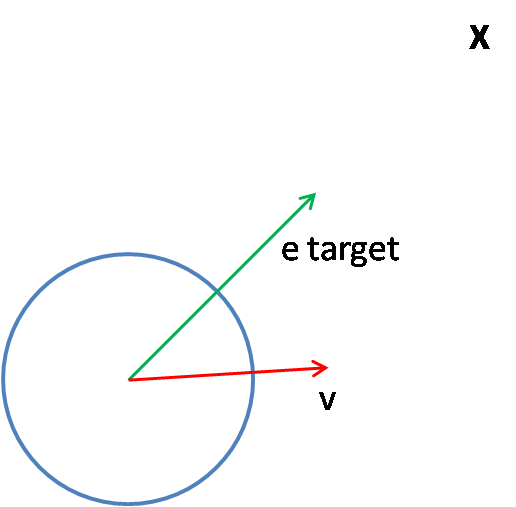
\includegraphics[scale=0.4]{pics/sfm/drivingforce} 
        \par
        \end{centering}
        \caption{\label{fig:driving-force} Driving force}
    \end{figure}
    
    The second term is known as the ``Social force''. It's calculated
    as follows:
    
    \begin{equation}
    \vec{F}_{S_{i}}=\sum_{j=1,j\ne i}^{N_{P}}Aexp(-\frac{\epsilon_{ij}}{B})\,\vec{e}_{ij}^{n}\label{eq:social-force}
    \end{equation}
    
    
    $\vec{F}_{S_{i}}$ represents the fact that a pedestrian keeps a certain
    distance to other pedestrians and borders.
    
    $N_{p}$ is the number of existing pedestrians.
    
    $A$ and $B$ are constants determined by simulations.
    
    $\epsilon_{ij}$ is the distance from $x_{i}$ towards $x_{j}$.
    
    $\vec{e}_{ij}^{n}$ is the unit vector from $x_{i}$ towards $x_{j}$.\\
    
    
    Fig. \ref{fig:Social-Force} shows equation \ref{eq:social-force} graphically.
    
    \begin{figure}[h]
        \begin{centering}
        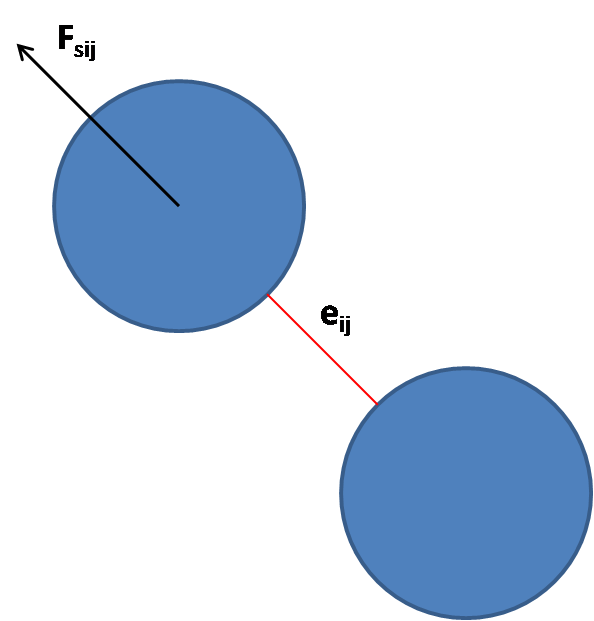
\includegraphics[scale=0.4]{pics/sfm/sf} \par
        \end{centering}
        \caption{Social Force\label{fig:Social-Force}}
    \end{figure}

    The third term is known as the ``Contact force''. It's calculated
    as follows:

    \begin{equation}
        \vec{F}_{G_{i}} = \sum_{j=1,j\ne i}^{N_{P}} [-\epsilon_{ij}k_{n}\vec{e}_{ij}^{n} + v_{ij}^{t} \epsilon_{ij} k_{t} \vec{e}_{ij}^{t}] \, g(\epsilon_{ij})
        \label{eq:granular-force}
    \end{equation}

    $\vec{F}_{G_{i}}$ represents the physical force that a pedestrian
    suffers when colliding with another object (pedestrian or wall).

    $k_{n}$ and $k_{t}$ are the normal and tangential friction coeficient
    respectively.

    $g$ is $0$ if $\epsilon_{ij}\leq0$ or $\epsilon_{ij}$ otherwise\\

    Fig. \ref{fig:colliding-pedestrians} shows \ref{eq:granular-force} graphically.
    
    \begin{figure}[h]
        \begin{centering}
        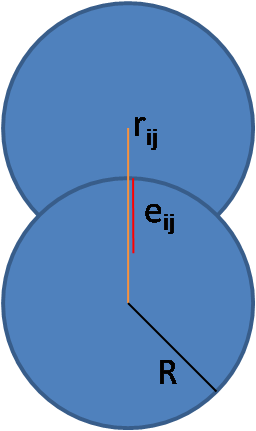
\includegraphics[scale=0.4]{pics/sfm/ganular} \par
        \end{centering}
        \caption{Colliding pedestrians\label{fig:colliding-pedestrians}}
    \end{figure}

    Afterwards $\vec{F}_{i}$ is calculated on each simulation step for
    each of the pedestrians and applied until all of them had reached
    their goal.
    
    Fixed parameter values:
    
    \begin{center}
    \begin{tabular}{|c|c|}
        \hline 
        Name  & Value\tabularnewline
        \hline 
        \hline 
        $A$  & $2000\,[N]$\tabularnewline
        \hline 
        $B$  & $0.08\,[m]$\tabularnewline
        \hline 
        $k_{n}$  & $1.2\,10^{5}\,[\frac{N}{m}]$\tabularnewline
        \hline 
        $k_{t}$  & $2.4\,10^{5}\,[\frac{kg}{m/s}]$\tabularnewline
        \hline 
        $\tau$  & $0.5\,[s]$\tabularnewline
        \hline 
    \end{tabular}
    \par
    \end{center}
    
    
    \subsection{Future Virtual Particle Model}
    
    Given that the SFM adds a fictional force on pedestrians, navigation
    is unnatural and doesn't resemble reality. SFM isn't validated using
    well known metrics for real-case scenarios such as the flow of pedestrians
    going out a door and the fundamental diagram \cite{key-pari2009}.
    
    In the FVPM, the social force in equation \ref{eq:driving-force}
    is eliminated and replaced with a dynamic driving force towards a
    short term objective, which is equal to equation \ref{eq:desired-direction}
    replacing $\vec{x}_{i}^{0}$ with $\vec{x_{i'}}$, where $\vec{x_{i'}}$
    is an estimation of the location of pedestrian $i$ in the near future.
    $i'$ will be called Future Virtual Particle. \\
    
    The presented work demanded a deep understanding of the problem in question, for which a 
    great study of related work was done. After that, we proposed various different models which
    were validated and reformed until it converged to this model, which validate against real
    world scenarios and metrics.
\section{The Model}
    
    \subsection{Hipotesis}
    
    The basic concepts below the model of pedestrian movement are the same
    as Helbin's \cite{key-helb1995,key-helb2000}:
    
    \begin{enumerate}
        \item The pedestrian wants to reach his goal in the shortest possible path. 
        \item The pedestrian's movement is influenced by other pedestrians. Depending
        on the distance between the two of them and the predicted trajectory,
        the pedestrian needs to change his route to be able to avoid obstacles. 
        \item Movement speed will be influenced by the presence of other pedestrians
        and obstacles. 
    \end{enumerate}
    
    \subsection{Geometrical definition}
    
    A pedestrian is defined as follows: 
    
    \begin{itemize}
        \item Circular shape
        
        Represents the personal space of a pedestrian. The value of the radio
        is generated randomly for each pedestrian. The range of values is
        distributed uniformly in $[0.25,0.29]$ $[cm]$ between pedestrians.
        
        \item Long term target
        
        Represented by a static area. It is considered as accomplished when
        the pedestrian touches this area. Multiple objectives could be defined
        in a list, in this case, each of them must be reached in order.
        
        \item Short term target
        
        Called future virtual particle (FVP), it represents a point at a relative
        distance from the pedestrian's center. It's a dynamic objective.
        
        It is defined as a $1\,[kg]$ mass. Not collisionable.
        
        \item Desired speed
        
        The speed the pedestrian would walk if he/she was alone. This represents
        the constant $v_{di}$ in ecuation \ref{eq:driving-force}. It takes
        a different value for each pedestrian. Varies with a uniform distribution
        between $[1.2,1.4]\,[m/s]$.
        
        \item Reaction distance ($RD$)
        
        
        Maximum distance between a pedestrian and his FVP, it represents the
        distance at which a real pedestrian would react from an obstacle.
    
    \end{itemize}
    
    \vspace{1cm}
    
    \begin{figure}[h]
        \centering{}
        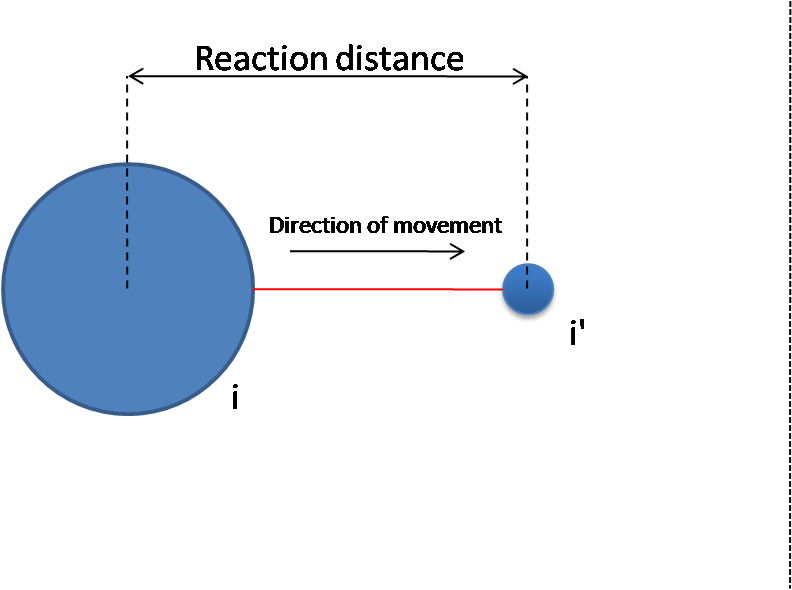
\includegraphics[scale=0.4]{pics/pedestrian-top} 
        \caption{\label{fig:pedestrian-geometry} Pedestrian $i$ and its FVP ($i'$).}
    \end{figure}
    
    The naming convention used for all vectors related to a pedestrian is shown in 
    fig. \ref{fig:pedestrian-vectors}.
    
    \begin{figure}[h]
        \centering{}
        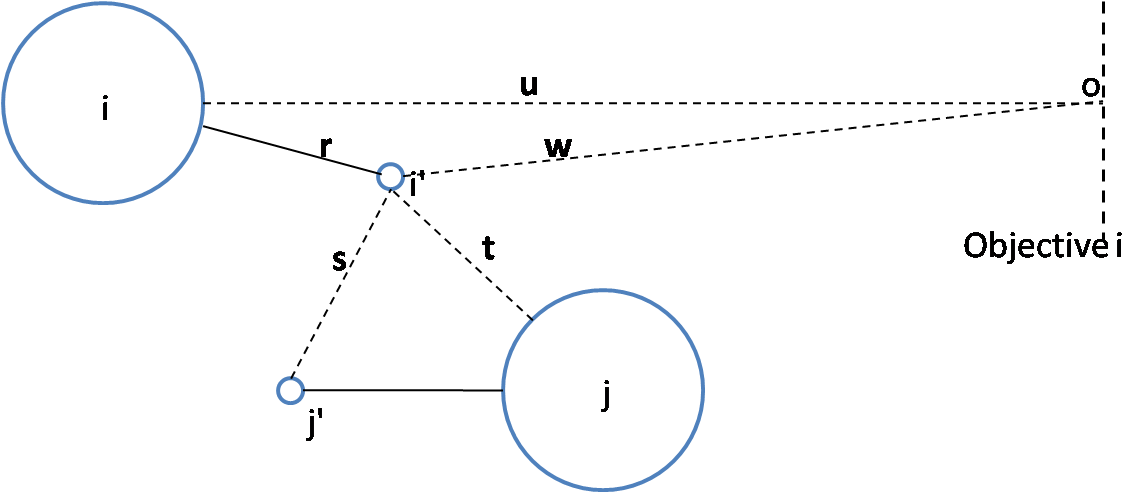
\includegraphics[scale=0.4]{pics/geometry}
        \caption{\label{fig:pedestrian-vectors} Vectors definitions}
    \end{figure}
    
    \subsection{Dynamics}
    
    \subsubsection{Force calculation}
    
    \begin{itemize}
    \item Dynamic of the FVP
        
        Each pedestrian has to reach the long term objective at some point,
        to ensure this, the FVP needs to be aligned with the shortest path
        to the long term objective $\mathbf{x_{o}}$. On the other hand, there
        are sometimes obstacles in the way, which will make this impossible,
        in this cases, the route will have to change depending on the situation.
        
        To model this situations, two types of forces act over the FVP: 
        
        \begin{itemize}
        \item Internal force \\
            
            For any pedestrian $i$, its internal force is
            
            \begin{equation}
                F_{i'}^{internal} = F_{i'}^{S1} + F_{i'}^{S2}
            \end{equation}
            where
            \[
                F_{i'}^{S1} = K_{1}(\theta_{i}) * (|\vec{r}| - RD) \hat{r}
            \]
            \[
                F_{i'}^{S2} = K_{2} * (\vec{x_{i'}} - (\vec{x_{i}} + \hat{x_{io}} RD))
            \]
            
            This force aligns the future on the path $\mathbf{x_{io}}$ and is modeled using 
            two springs $S_1$ and $S_2$:\\
            
            $S_1$ starts on $\mathbf{x_{i}}$, ends on $\mathbf{x_{i'}}$ and 
            has a stationary distance of $RD$ with a spring constant $K_{1}(\theta)$ 
            where $\theta$ is the angle between $\mathbf{u}$ and $\mathbf{r}$. With this 
            spring the FVP will tend to always be at $RD$ distance from the pedestrian.
            Because a pedestrian always tries to reach his goal in the shortest
            possible path (hypothesis 1), if it has to take a big detour of his
            ideal path, it will try to reduce his velocity drastically in order
            to avoid making a long travel. To recreate this, the spring constant
            has to be dependant of the deviation angle.
            \[
                K_{1}(\theta) = \frac{K_{1c}}{\theta}
            \]
            where $K_{1c}$ is a constant value.
            
            $S_2$ starts on $\mathbf{x_{i'}}$ and ends on $\mathbf{x_{i}} + RD\mathbf{{\hat{x}_{io}}}$
            with a spring constant $K_{2c}$. Setting a greater $K_{2c}$ spring constant 
            will force a straighter path but may result in more collisions. In order to 
            avoid an oscillatory movement, a damping $\gamma$ is added to the spring $S_2$. \\
            Fig. \ref{fig:internal-forces} shows the internal forces that a FVP $i'$ suffers 
            because it has to be aligned with the pedestrian's position $\mathbf{x_{i}}$ and the long 
            term objective $\mathbf{x_{o}}$ but also at distance $RD$ from $\mathbf{x_{i}}$.

            \begin{figure}[H]
                \centering{}
                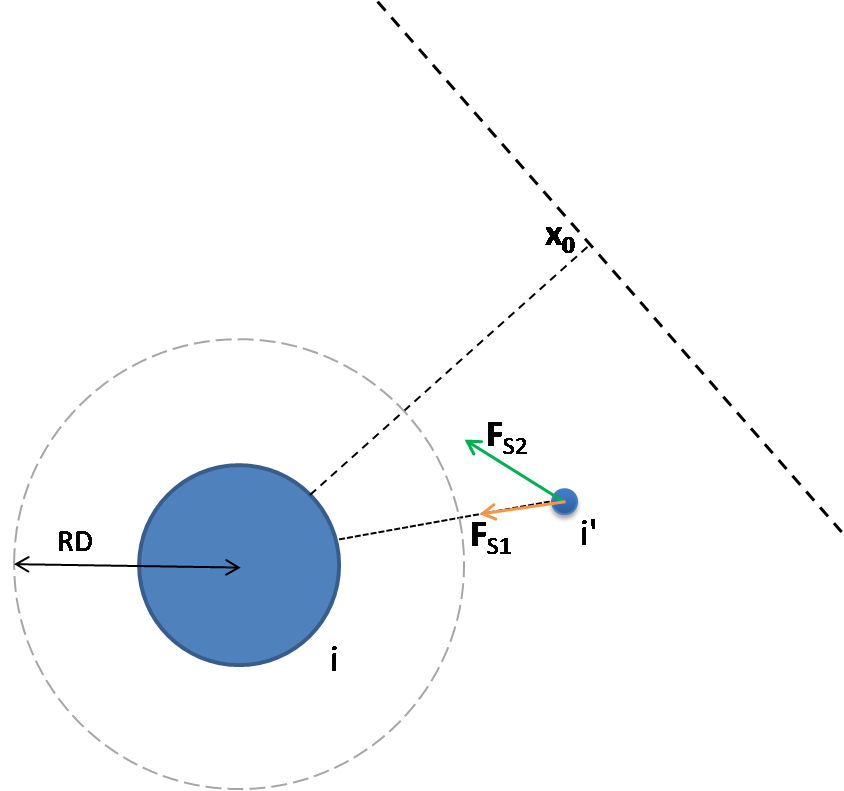
\includegraphics[scale=0.35]{pics/pedestrian-internal-forces}
                \caption{\label{fig:internal-forces} Internal forces}
            \end{figure}

        \item External forces \\
            
            This force will produce avoidance movements when obstacles are detected
            on the path. The equation for the external force that affects the FVP $i'$ is
            \begin{equation}
                F_{i'}^{external} = FF_{i'} + FP_{i'} + FW_{i'} \label{eq:externalforce}
            \end{equation}
            where 
            \[
                FF_{i'} = \sum_{j}^{N}(\alpha_{ff}e^{-s/\beta_{ff}})
            \]
            \[
                FP_{i'} = \sum_{j}^{N}(\alpha_{fp}e^{-t/\beta_{fp}})
            \]
            \[
                FW_{i'} = \sum_{k}^{walls}(\alpha_{fw}e^{-\zeta_{k} /\beta_{fw}})
            \]
            having $\zeta_{k} = |x_{i'} - x_{k}|$; $x_{k}$ being the closest point from wall 
            $k$ to $x_{i'}$. \\
            $\alpha$ and $\beta$ are constants. \\
            The term $FF_{i'}$ in equation \ref{eq:externalforce} acts as a repulsion force 
            between $i'$ and $j'$, resulting in the avoidance of a future collision. The term 
            $FP_{i'}$ in equation \ref{eq:externalforce} uses this same principle but 
            calculates the repulsion  force between $i'$ and $j$. The term $FW_{i'}$ in equation 
            \ref{eq:externalforce} adds the repulsion against walls,  using the closest point 
            between $i'$ and the wall. \\
            This force is only applied to each the pedestrian $j$ ($j\neq i$)
            who is in the range of sight of pedestrian $i$. The restriction
            is verified using the following condition:
            \[
                \mathbf{r_{ii'}}\bullet\mathbf{r_{ij}} > 0
            \]
            The condition represents the fact that pedestrians make decisions
            based only on obstacles in his range of vision. \\
            Fig. \ref{fig:external-forces} shows the external forces
            that a FVP $i'$ suffers because of another pedestrian ($j$)
            and also the direction in which $i$ desires to move.

            \begin{figure}[H]
                \centering{}
                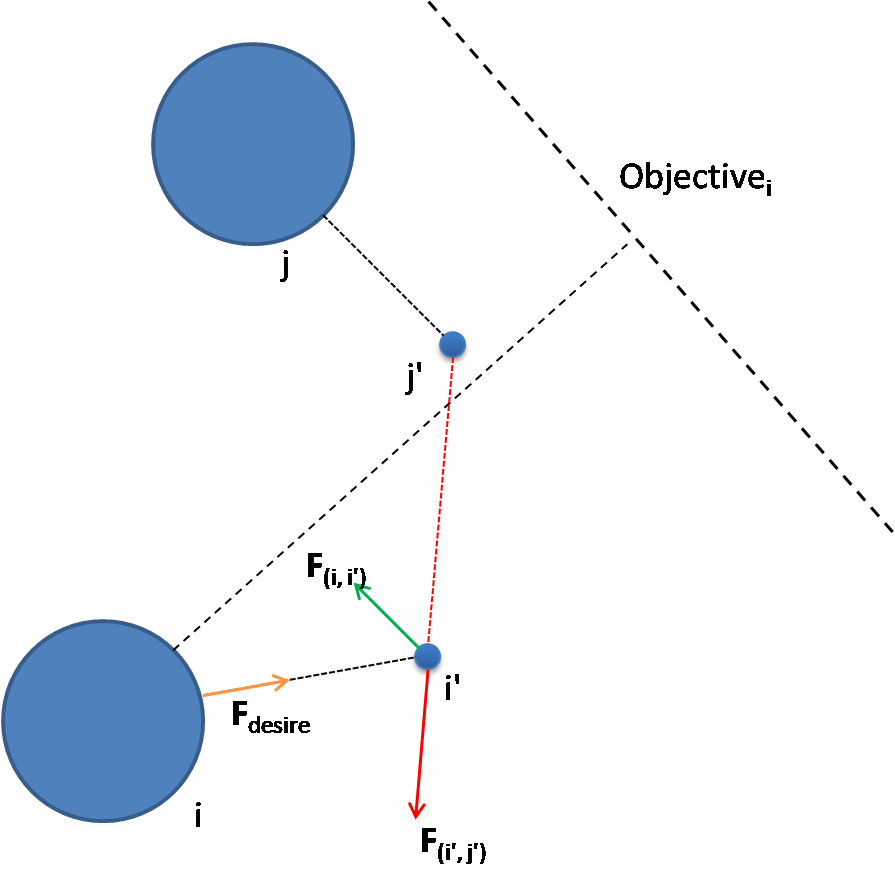
\includegraphics[scale=0.35]{pics/pedestrian-top-forces}
                \caption{\label{fig:external-forces} External forces}
            \end{figure}

        \end{itemize}

        After this, $F_{i'}$ is computed by adding all the terms.

        \begin{equation}
            F_{i'} = F_{i'}^{external} + F_{i'}^{internal} \label{eq:future-force}
        \end{equation}
        
        To avoid high symmetry situations, a small noise is added to $F$. 
        This noise is calculated by taking a random value $s$ with a random distribution from $\{-1, 1\}$
        and applying:
        \[
            M=\left(\begin{array}{cc}
            0 & -s\\
            s & 0
            \end{array}\right)
        \]
        in
        \[
            F'_{i'} = F_{i'} + F_{i'} * M
        \]
        
        Finally, movement equations are applied using $F'_{i'}$.
    
    \item Dynamic of the pedestrian
        
        The driving force $\vec{F}_{d_{i}}$ makes the pedestrian tend to move towards his FVP at velocity $v_{di}$
        \[
            \vec{F}_{d_{i}} = m_{i}\frac{|v_{di}|\frac{\vec{r}}{RD} - \vec{v}_{i}}{\tau}
        \]
        where $\tau=0.5$\\
    
        It is important to note that the only deviation from the
        SFM in this equation is the $k\vec{e}_{i}$ term. As described above,
        this model focuses on improving the SFM through dynamically adjusting
        the desired velocity.   
    
    \end{itemize}
    
    \subsubsection{Algorithm}
    
    The pedestrian movement is calculated in four steps: 
    \begin{enumerate}
        \item Calculate forces for each FVP. 
        \item Calculate forces for each pedestrian. 
        \item Update positions for each FVP. 
        \item Update positions for each pedestrian. 
    \end{enumerate}

\section{Calibration}

    \subsection{Scenarios}
        
        The test scenarios where crossing and hallway for they present the
        main types of symmetry (90 degrees and 180 degrees respectively). \\
        
        Hallway scenario: A $15[m]$ by $4[m]$ hallway. Pedestrians are generated
        from each end at a pace of 1 pedestrian per second with the other
        end as target. \\
         This scenario is shown in fig. \ref{fig:hallway-scenario}.
        
        \begin{figure}[H]
            \centering{}
            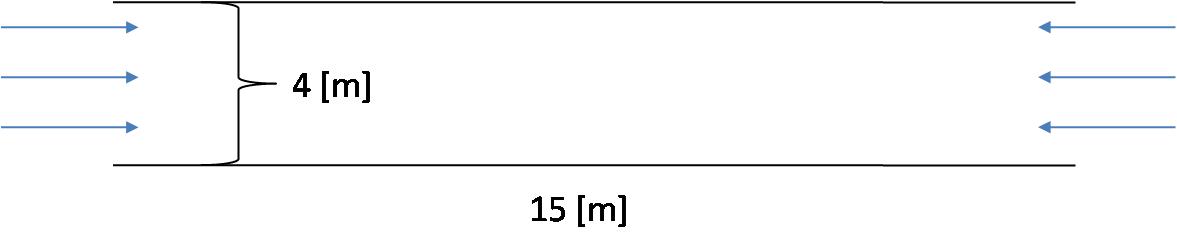
\includegraphics[scale=0.35]{pics/scenarios/hallway}
            \caption{\label{fig:hallway-scenario}Hallway Scenario}
        \end{figure}
        
        Crossing scenario: Two hallways of $25[m]$ length by $5[m]$ width
        put together in the center forming a cross. Pedestrians are generated
        from the top, targeting the bottom, and from the right end, targeting
        the left end, at a pace of 1 pedestrian per second. \\
         This scenario is shown in fig. \ref{fig:cross-scenario}.
        
        \begin{figure}[H]
            \centering{}
            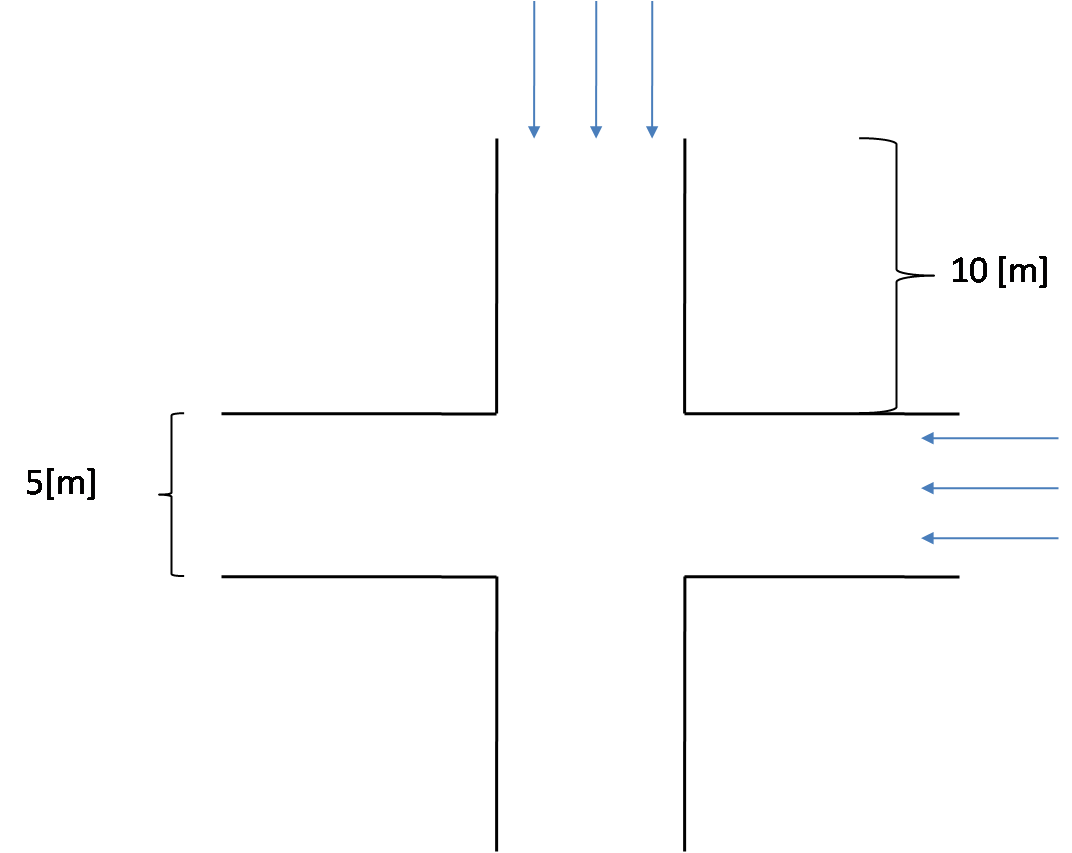
\includegraphics[scale=0.3]{pics/scenarios/cross}
            \caption{\label{fig:cross-scenario} Cross Scenario}
        \end{figure}
    
        Room evacuation: A $20x20[m]$ room with a single exit door
        centered at the bottom. At the beginning, a fixed number of pedestrians are 
        distributed across the room. Each of them targeting the exit door. When the 
        first pedestrian exits the room, a counter starts, and when the last one 
        crosses, it stops. This way we can measure the flow of pedestrians leaving a 
        room, which is known to be between $1$ and $4$ [p/m/s] for pedestrians 
        without emergencies \cite{key-pari2009}. \\
        The door size will be tested using the following measures: $1.2[m]$, $1.5[m]$ and $1.8[m]$. \\
        This scenario is shown in fig. \ref{fig:room}.
        \begin{figure}[H]
            \centering{}
            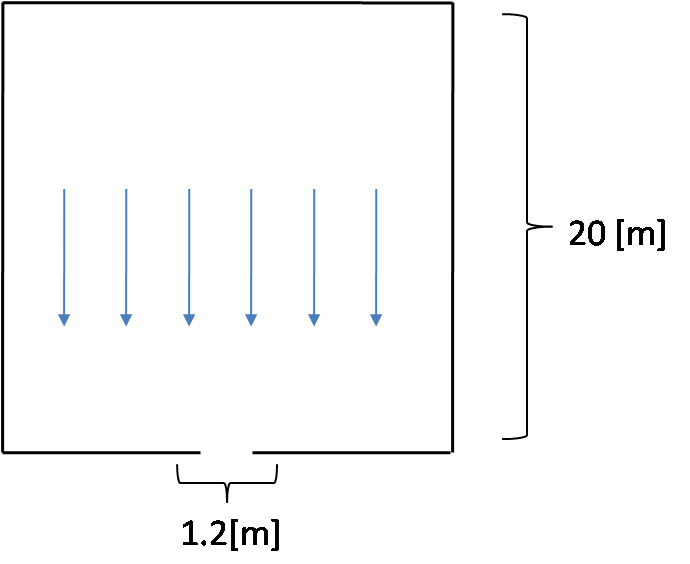
\includegraphics[scale=0.3]{pics/scenarios/room}
            \caption{\label{fig:room} Room Scenario}
        \end{figure}
    
    \subsection{Metrics}
        The metrics used to validate and verify the model against the hallway and 
        crossing scenarios are defined as follows:
        
        \begin{enumerate}
            \item Number of collisions:

            \begin{eqnarray*}
                \sum_t\sum_i\sum_j collides(i,j)/2
            \end{eqnarray*}
            
            where
            
            \begin{eqnarray*}
            collides(i,j,t) = touching(i,j,t) (1 - touching(i,j,t-1))\\
            \end{eqnarray*}
            
            \begin{eqnarray*}
            touching(i,j,t) = 
            \left \{
                \begin{tabular}{cc}
                $0$ & if $t<=0$\\
                $1$ & if $x_i-x_j<R_i+R_j$\\
                $0$ & if not
                \end{tabular}
            \right .
            \end{eqnarray*}
            
            \item Amount of collisions per instant: The equation for this metric is
            defined as:
             
            \begin{eqnarray*}
                \sum_t\sum_i\sum_j touching(i,j)/2
                %\sum\#\{(i,j)\,/\, id_{i}<id_{j}\wedge\\
                %x_{i,t_{n}}-x_{j,t_{n}}<R_{i}+R_{j}\}\,\,\forall t_{n}
            \end{eqnarray*}
            
            \item Average walking speed:
             
            \begin{eqnarray*}
                \sum_{t=0}^T((\sum_{i=0}^N v_i)/N)/T
            \end{eqnarray*}
            
            \item Average travel time: The average time that a pedestrian takes to
            reach the goal. This is calculated only for pedestrians who reach the goal
            before the simulation ends.
            
            \item Average travel distance: The average distance that pedestrians traveled
            until it reached the goal. This is calculated only for pedestrians who reach the goal
            before the simulation ends.
             
            \item Average turn angle: The average angle turned by a pedestrian until
            it reached the goal. This is calculated only for pedestrians who reach the goal
            before the simulation ends.\\
            where the turn angle is:
             
            \begin{eqnarray*}
                \arccos(v_{t_{n}}\bullet v_{t_{n-1}}/|v_{t_{n}}\bullet v_{t_{n-1}}|)
            \end{eqnarray*}
            
        \end{enumerate}
        
        The metric used for the room evacuation scenario is:
        
        \begin{enumerate}
            \item Escape flow: The amount of pedestrians coming out of the room by second.
            \begin{eqnarray*}
                \frac{N}{\Delta T}
            \end{eqnarray*}
            
            where $\Delta T$ is the time when the last pedestrian exits minus
            the time when the first pedestrian exits.
        
        \end{enumerate}
    
        All results were compared to the SFM model \cite{key-helb2000}.

    \subsection{Values}

        To calibrate the model, runs with varying parameters were made.
        % MARSE TRADUCIR: Los parametros fueron buscados de manera exhaustiva usando una tecnica de barrido.
        % Se variaron los parametros FVP-FVP: $\alpha$ y $\beta$ realizando incrementos de a 0.2

        All runs used Euler method with a step of $\frac{1}{1000}$ $[s]$. For each scenario 
        and parameter combination, $10$ runs were made 
        and their metric results averaged and compared against each set of parameters. \\
        After numerous iterations of this process, this are the parameters which best fit all scenarios:
        
        \begin{itemize}
            \item Pedestrian 
            
            \begin{itemize}
                \item $K_{1}=80$ {[}N/m{]}, 
                \item $\gamma=10$ 
                \item $K_{2}=100$ {[}N/m{]} 
            \end{itemize}
            \item FVP-FVP interaction 
            
            \begin{itemize}
                \item $\alpha=1000$ 
                \item $\beta=[0.4,\,0.6]$ (Uniform distribution) 
                \end{itemize}
            \item Pedestrian-FVP interaction 
            
            \begin{itemize}
                \item $\alpha=1000$ 
                \item $\beta=0.1$ 
            \end{itemize}
            \item FVP-Wall interaction 
            
            \begin{itemize}
                \item $\alpha=10000$ 
                \item $\beta=0.1$ 
            \end{itemize}
        \end{itemize}

\section{Results}
    
    All results for each metric for the crossing scenario are presented on table \ref{table:metric-crossing}:
    
    \begin{table}[H]
        \begin{centering}
            \begin{tabular}{|c|c|c|}
                \hline 
                Metric  & {\scriptsize{FVPM}} & {\scriptsize{SFM ($\alpha=2000,\,\beta=0.08$)}}\tabularnewline
                \hline 
                \hline 
                $1$  & {\scriptsize{$15.0\pm4.3$}} & {\scriptsize{$23.2\pm6.4$}}\tabularnewline
                \hline 
                $2$  & {\scriptsize{$158.2\pm60.6$}} & {\scriptsize{$57.2\pm18.8$}}\tabularnewline
                \hline 
                $3$  & {\scriptsize{$1.26\pm0.02$ $[m/s]$}} & {\scriptsize{$1.28\pm0.01$ $[m/s]$}}\tabularnewline
                \hline 
                $4$  & {\scriptsize{$17.61\pm0.27$ $[s]$}} & {\scriptsize{$17.33\pm0.06$ $[s]$}}\tabularnewline
                \hline 
                $5$  & {\scriptsize{$22.61\pm0.07$ $[m]$}} & {\scriptsize{$22.52\pm0.07$ $[m]$}}\tabularnewline
                \hline 
                $6$  & {\scriptsize{$103.35\pm32.81$ $[rad]$}} & {\scriptsize{$193.06\pm20.44$ $[rad]$}}\tabularnewline
                \hline 
            \end{tabular}
        \par\end{centering}
        \caption{Results for crossing scenario \label{table:metric-crossing}}
    \end{table}

    Metrics for the crossing scenario don't present noticeable improvements over the SFM.
    The one improvement is the average turn angle, which can be recognized by looking
    and comparing the two models. The SFM presents a much more unnatural navigation than
    the FVPM.
    
    \begin{figure}[H]
        \begin{centering}
            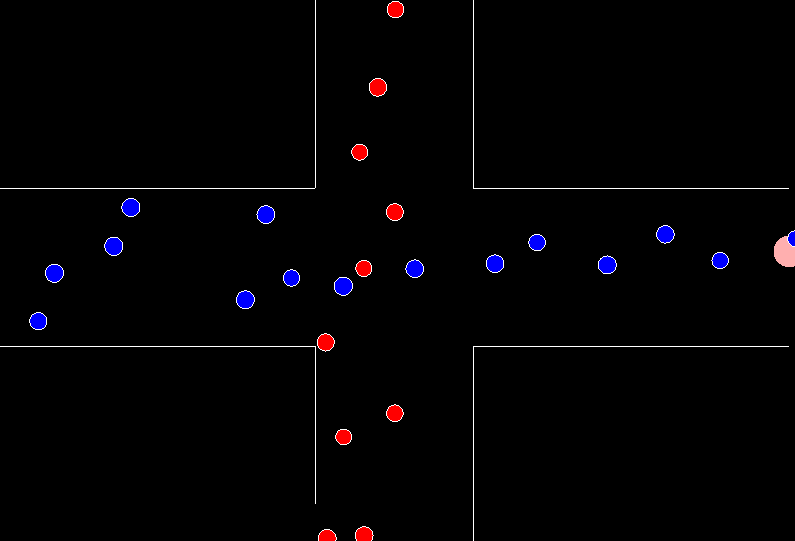
\includegraphics[width=6cm]{pics/program/crossing-no-future} 
            \par
        \end{centering}
        \caption{\label{fig:crossing-no-future}Crossing visualization}
    \end{figure}

    \begin{figure}[H]
        \centering{} 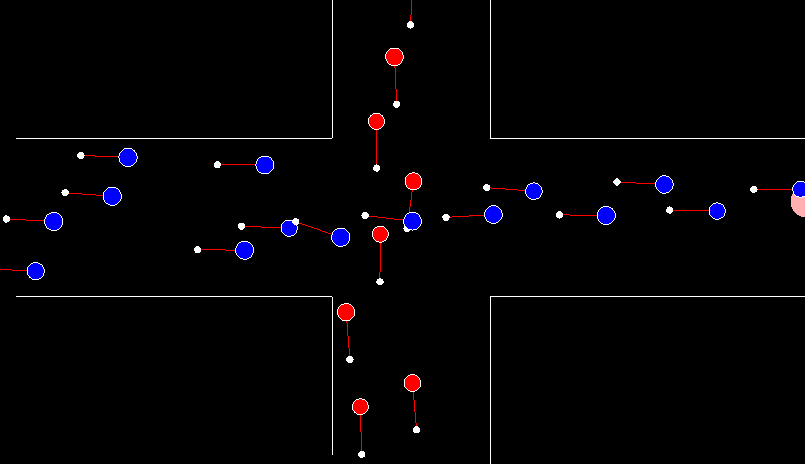
\includegraphics[width=6cm]{pics/program/crossing-future}
        \caption{\label{fig:crossing-future}Crossing visualization with visible future}
    \end{figure}
    
    \vspace{1cm}
    All results for each metric for the hallway scenario are presented on table \ref{table:metric-hallway}:
    \begin{table}[H]
        \begin{centering}
			\begin{tabular}{|c|c|c|}
				\hline 
				Metric  & {\scriptsize{FVPM}} & {\scriptsize{SFM ($\alpha=2000,\,\beta=0.08$)}}\tabularnewline
				\hline 
				\hline 
				$1$  & {\scriptsize{$7.8\pm5.3$}} & {\scriptsize{$20.8\pm8.5$}}\tabularnewline
				\hline 
				$2$  & {\scriptsize{$53.8\pm29.5$}} & {\scriptsize{$85.2\pm32.3$}}\tabularnewline
				\hline 
				$3$  & {\scriptsize{$1.27\pm0.01$ $[m/s]$}} & {\scriptsize{$1.04\pm0.08$ $[m/s]$}}\tabularnewline
				\hline 
				$4$  & {\scriptsize{$13.15\pm0.06$ $[s]$}} & {\scriptsize{$18.17\pm2.12$ $[s]$}}\tabularnewline
				\hline 
				$5$  & {\scriptsize{$17.13\pm0.05$ $[m]$}} & {\scriptsize{$19.16\pm0.83$ $[m]$}}\tabularnewline
				\hline 
				$6$  & {\scriptsize{$109.88\pm6.22$ $[rad]$}} & {\scriptsize{$1431.94\pm436.44$ $[rad]$}}\tabularnewline
				\hline 
			\end{tabular}
        \par\end{centering}
        \caption{Results for hallway scenario \label{table:metric-hallway}}
    \end{table}

    In the hallway scenario, great improvements in behaviour and metrics were achieved.
    Every metric was beaten by the new model with considerable changes. The FVPM
    removes the bouncing of pedestrians which is typical of the SFM in this
    scenario and gives way to the forming of natural pathways for pedestrians.
    
    \begin{figure}[H]
        \begin{centering}
        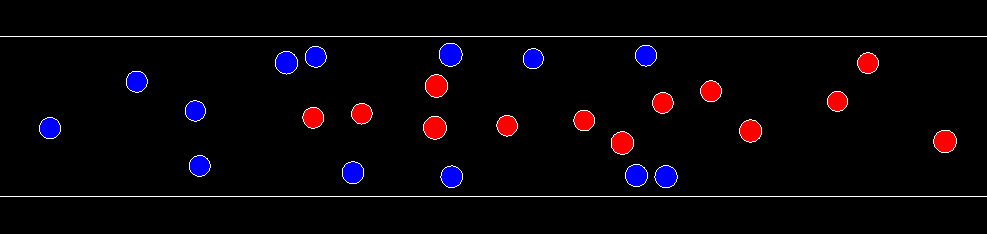
\includegraphics[width=6.5cm]{pics/program/hallway-no-future} 
        \par\end{centering}
        
        \caption{\label{fig:hallway-no-future}Hallway visualization}
    \end{figure}

    \begin{figure}[H]
        \begin{centering}
        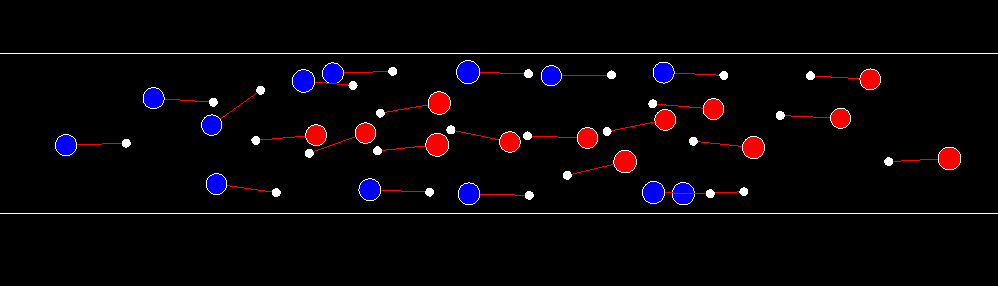
\includegraphics[width=6.5cm]{pics/program/hallway-future} 
        \par\end{centering}
        
        \caption{\label{fig:hallway-future}Hallway visualization with visible future}
    \end{figure}
    
    The number of collisions is decreased compared to the SFM. The fact
    that the time of collision (metric \#2) is bigger than in the SFM,
    resembles reality, pedestrians don't shoot out at great velocities
    when colliding. The average travel distance is similar in the crossing
    scenario but much smaller in the hallway, this shows the problem of
    SFM in high symmetry scenarios (inverse velocities). \\
     Each pedestrian turns (in average) $10\%$ less with the FVPM than
    with the SFM in both scenarios. \\

    For the escape room scenario, all 9 combinations for the number of pedestrians in [$100$, $150$, $200$] 
    and the door sizes in [$1.2$, $1.5$, $1.8$] where run.
    Before presenting the results, two definitions need to be defined:
    \begin{itemize}
        \item Pedestrian flow: This is the amount of pedestrians that left the room
        per unit of time. It is defined as: 
        \[
            Q=\frac{\triangle N}{\triangle T}\,\,[Pedestrian/s]
        \]
         
        \item Pedestrian specific flow: This is the amount of pedestrians that left
        the room per unit of time per unit of distance. It is defined as:
        \[
            Q_{s}=\frac{\triangle N}{\triangle T*door\_width}\,\,[Pedestrian/s/m]
        \]
    \end{itemize}

    
    The average pedestrian flow ($Q_avg$) was taken by averaging the results of $5$ simulations for each configuration.\\
    The results are shown on fig. \ref{fig:room-flow-100}, fig. \ref{fig:room-flow-150} and fig. 
    \ref{fig:room-flow-200}.

    \begin{figure}[H]
        \begin{centering}
        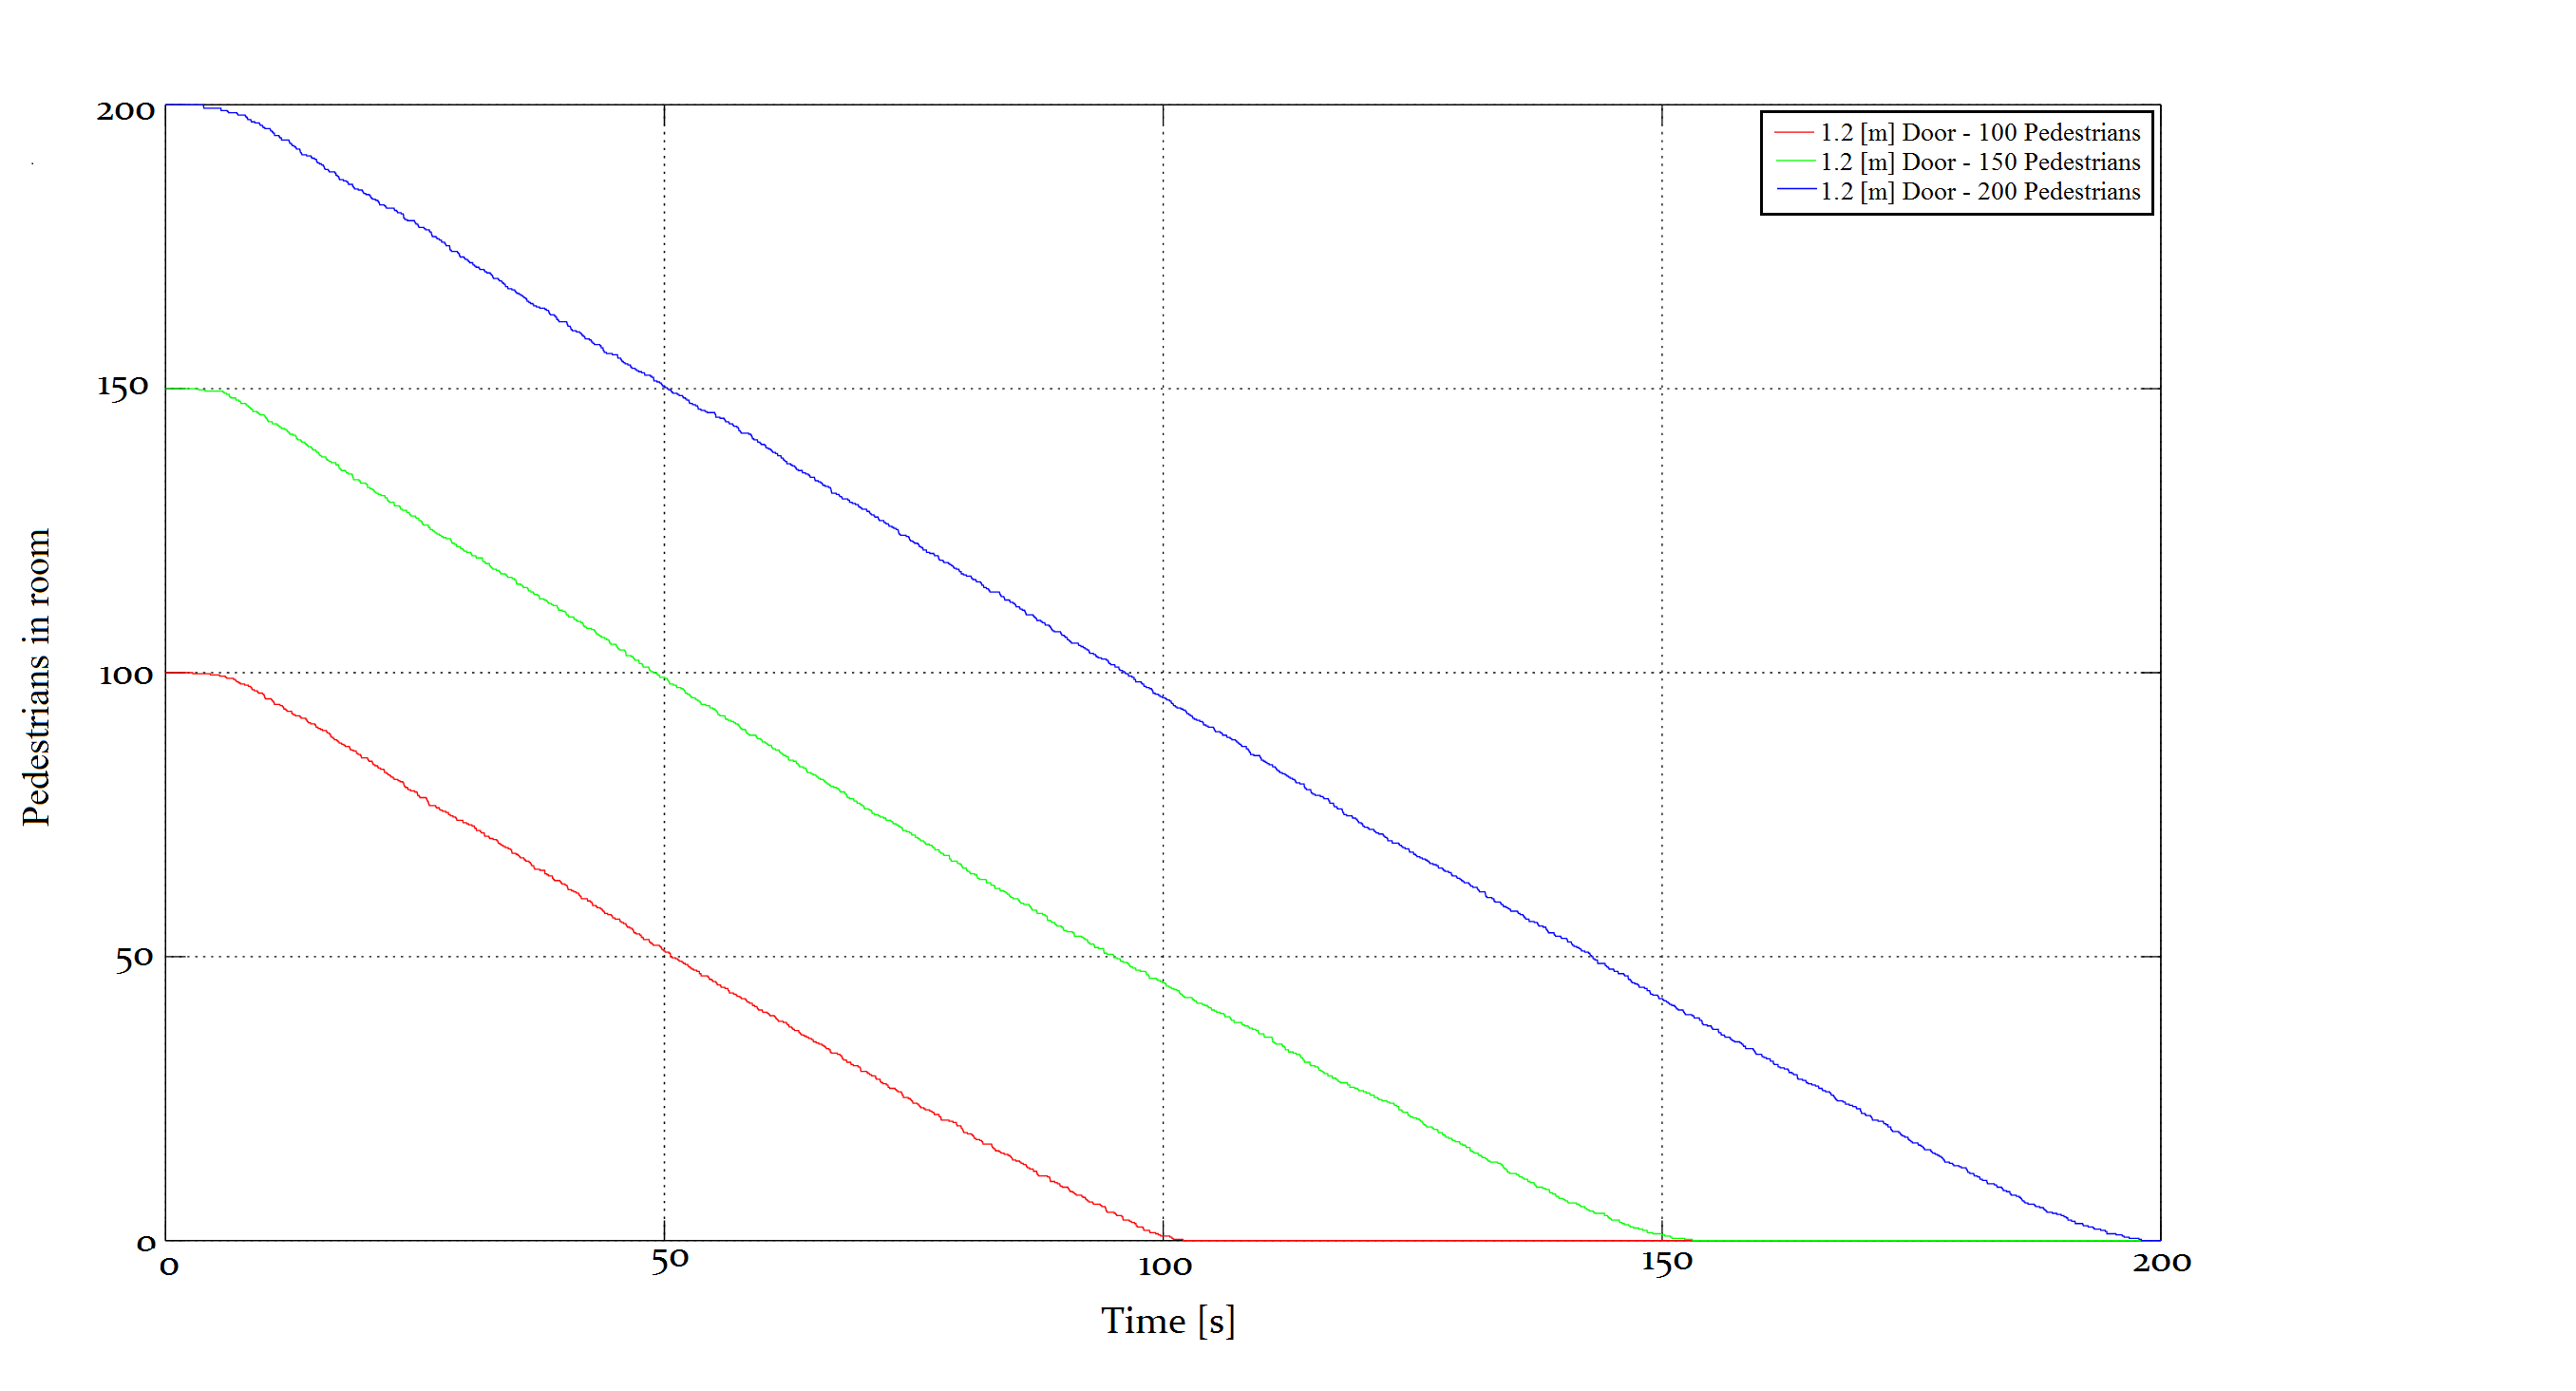
\includegraphics[scale=0.2]{pics/flow/12door} 
        \par\end{centering}
        \caption{\label{fig:room-flow-100}Room evacuation with $1.2$ $[m]$ door}
    \end{figure}
    
    \begin{figure}[H]
        \begin{centering}
        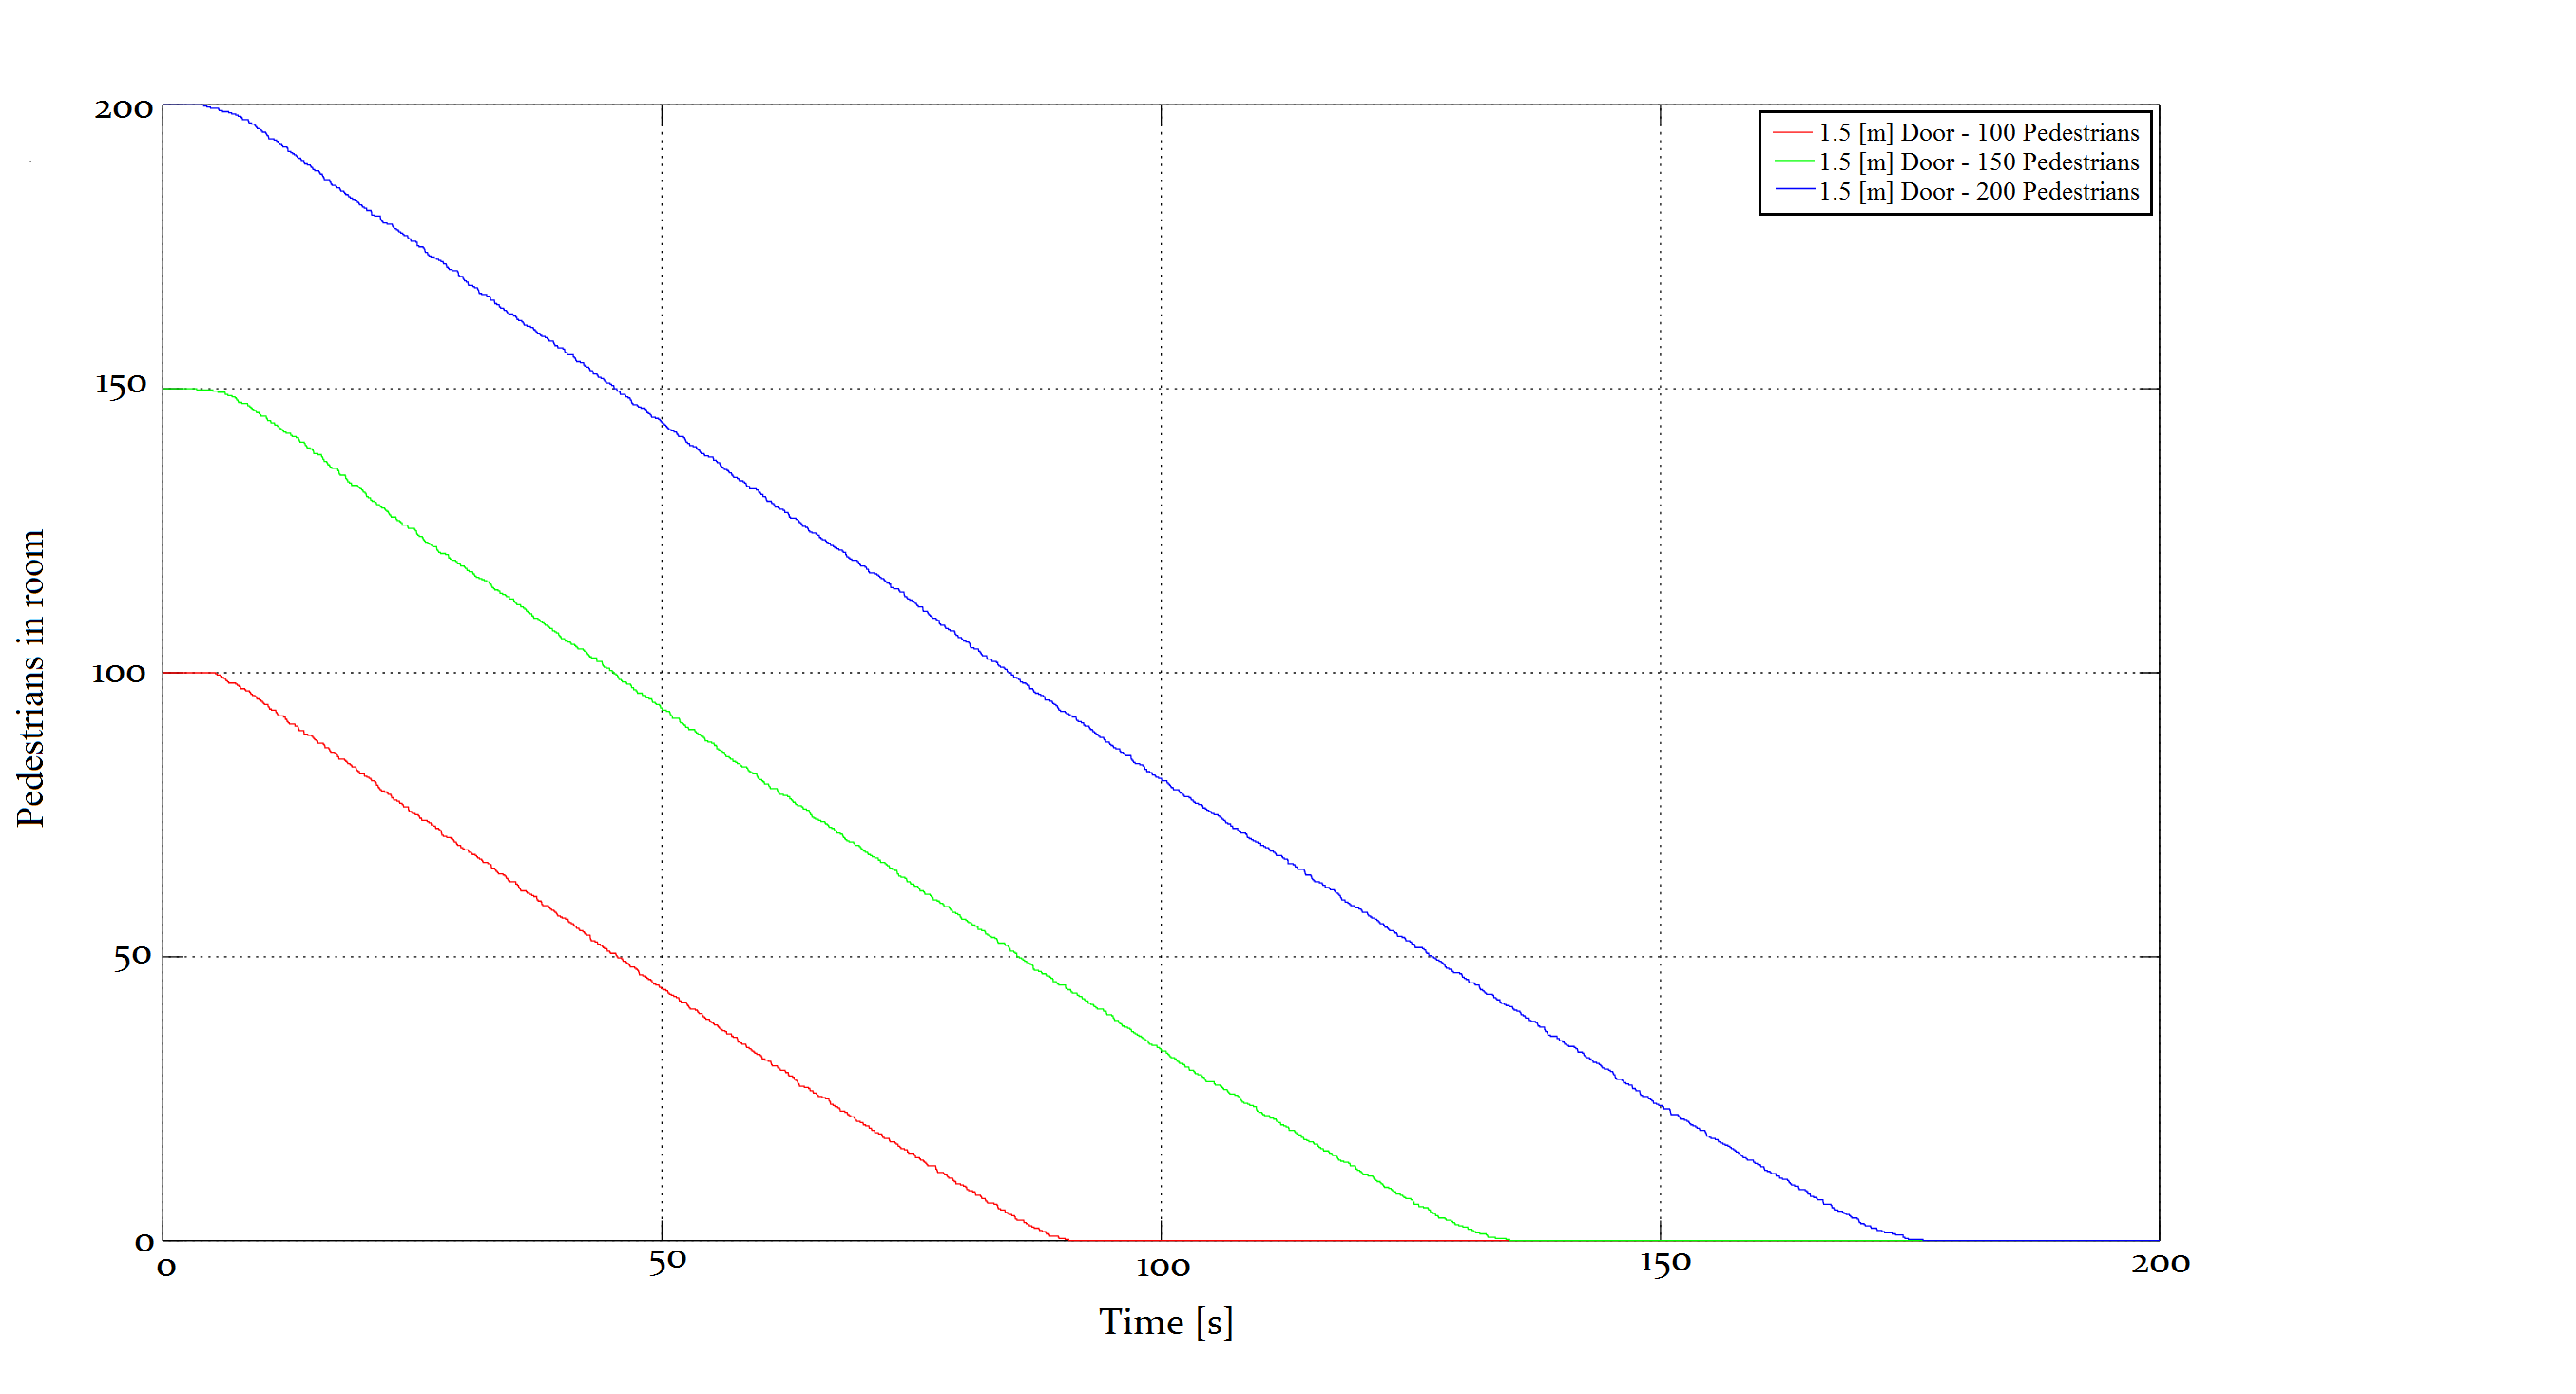
\includegraphics[scale=0.2]{pics/flow/15door} 
        \par\end{centering}
        \caption{\label{fig:room-flow-150}Room evacuation with $1.5$ $[m]$ door}
    \end{figure}
    
    \begin{figure}[H]
        \begin{centering}
        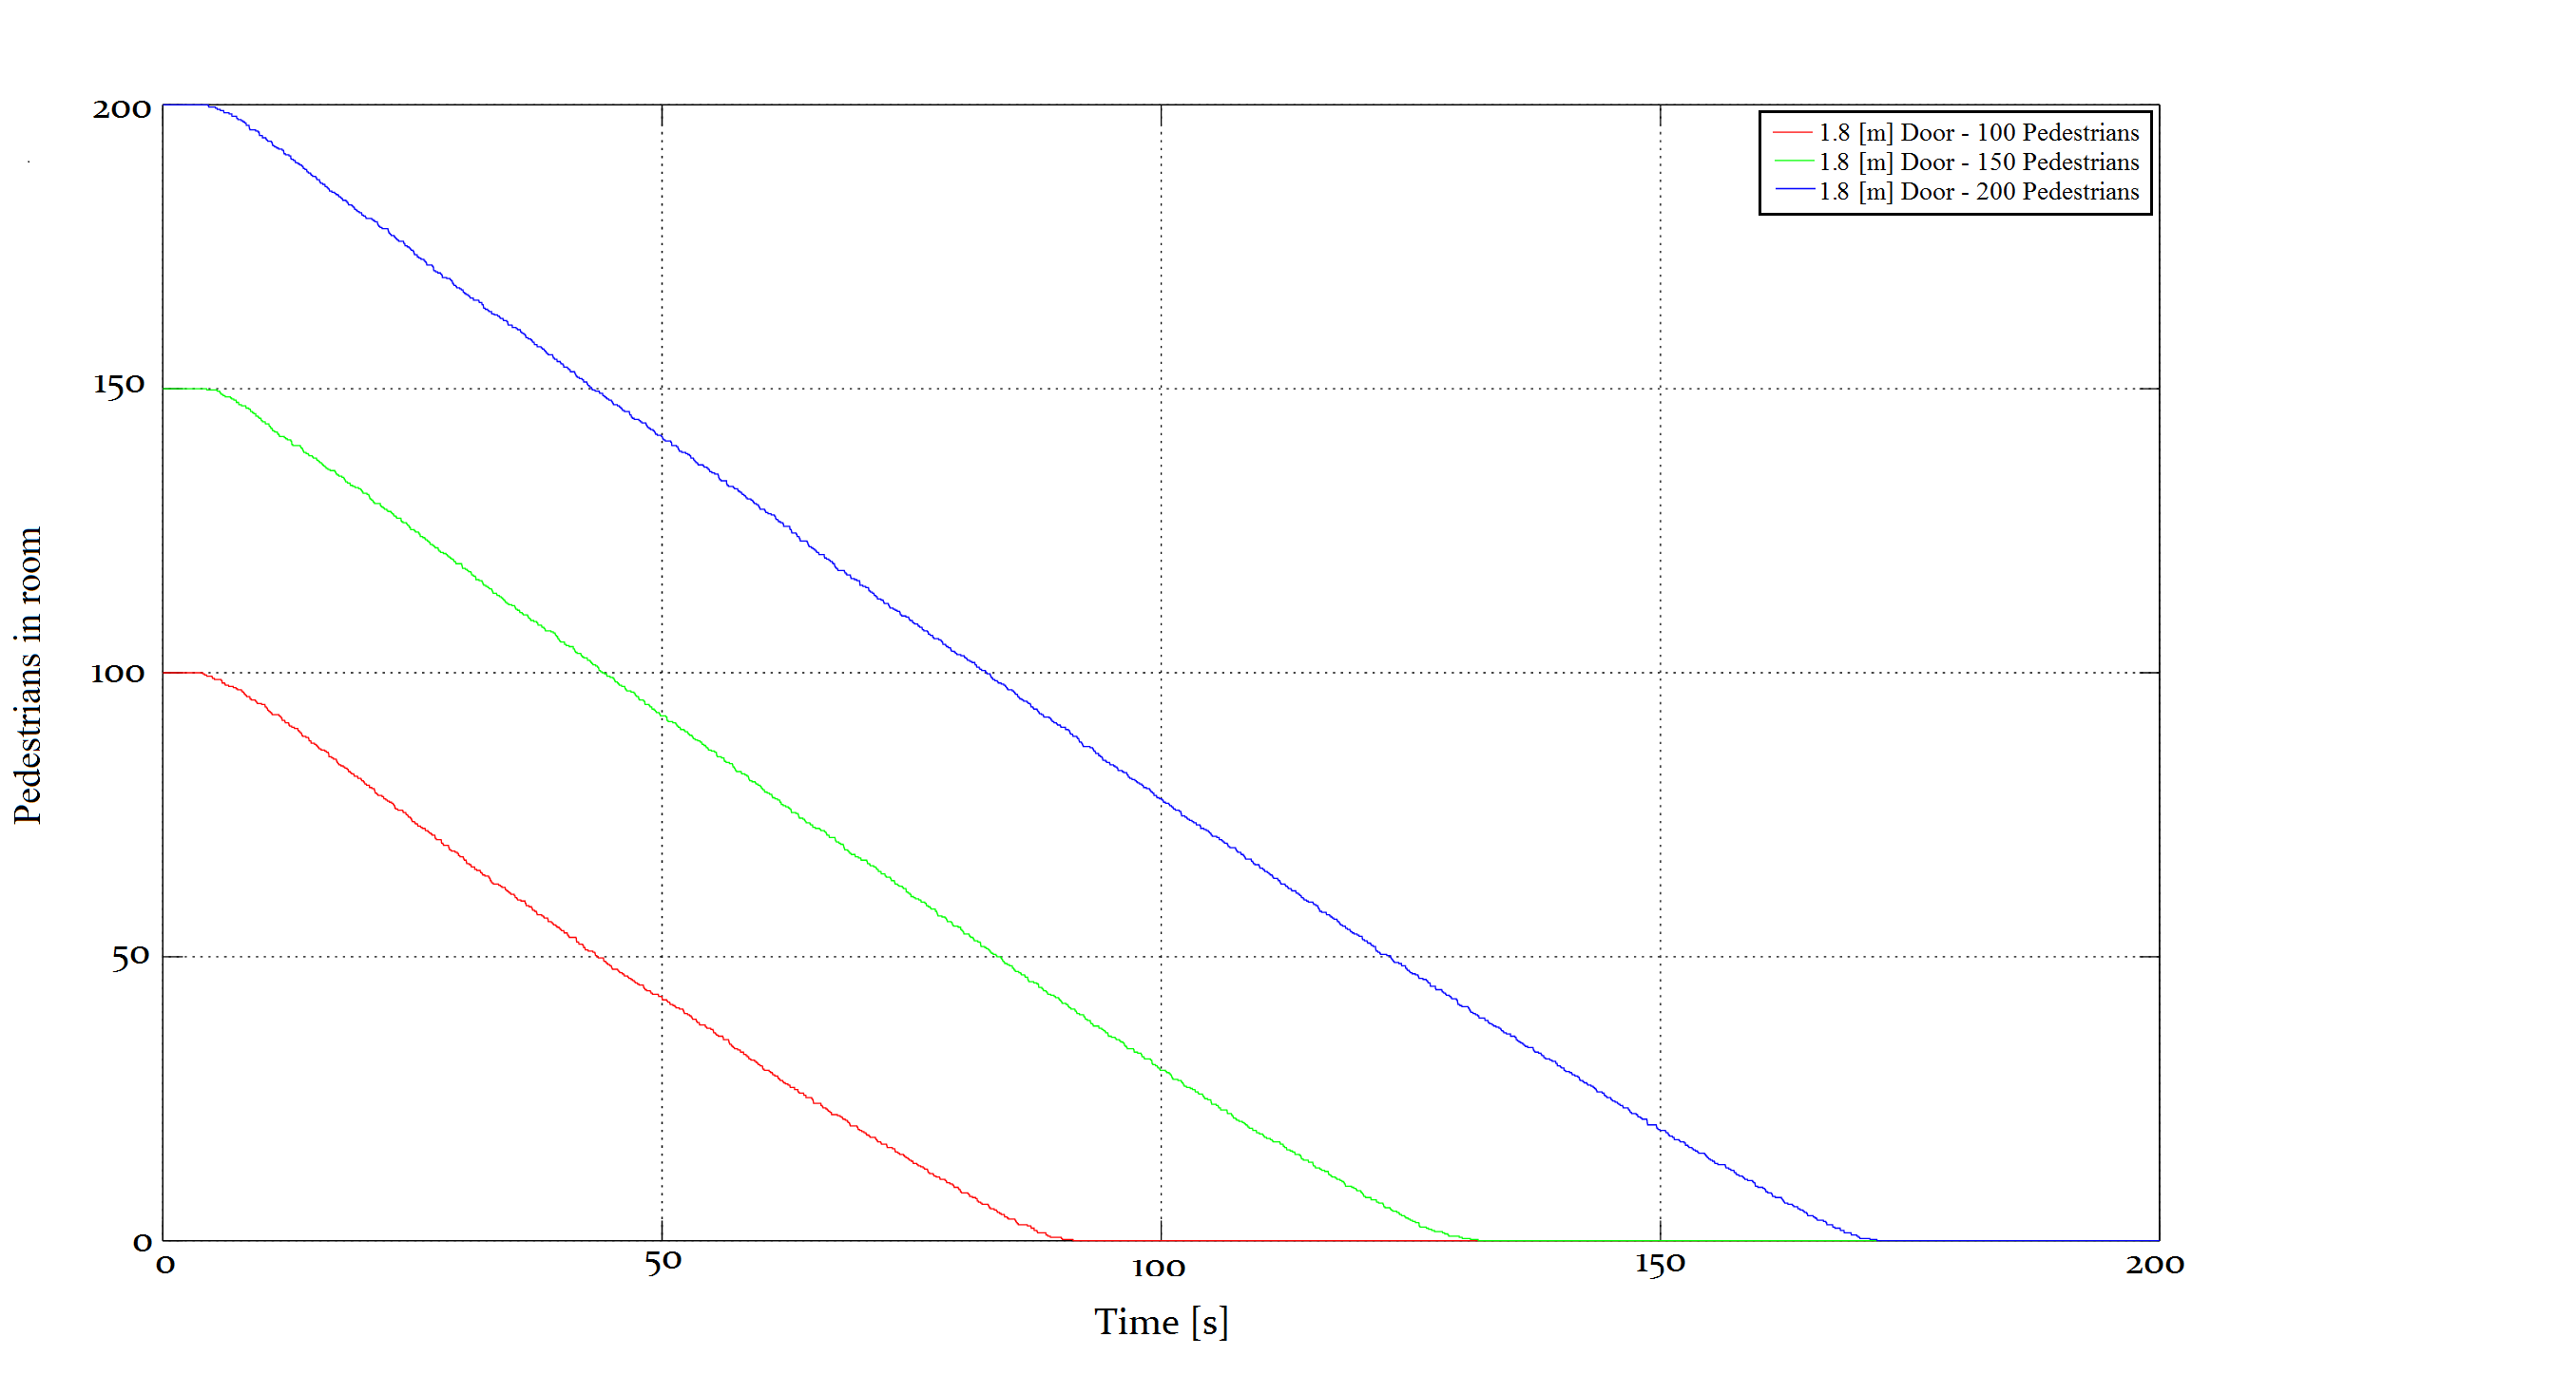
\includegraphics[scale=0.2]{pics/flow/18door} 
        \par\end{centering}
        \caption{\label{fig:room-flow-200}Room evacuation with $1.8$ $[m]$ door}
    \end{figure}
    
    The escape flow for each configuration was calculated using octave's $polyfit$ using a 
    grade $1$ polygon and the slopes for each door size are as follows:

    \begin{table}[H]
        \begin{centering}
        \begin{tabular}{|c|c|c|c|}
        \hline 
        N \textbackslash{} Door size & $1.2$ & $1.5$ & $1.8$\tabularnewline
        \hline 
        \hline 
        $100$ & $1.02$ & $1.05$ & $1.05$\tabularnewline
        \hline 
        $150$ & $1.17$ & $1.18$ & $1.18$\tabularnewline
        \hline 
        $200$ & $1.20$ & $1.22$ & $1.23$\tabularnewline
        \hline 
        \end{tabular}
        \caption{Escape room configurations \label{tbl:room-runs}}
        \end{centering}
    \end{table}

    \begin{figure}[H]
        \begin{centering}
        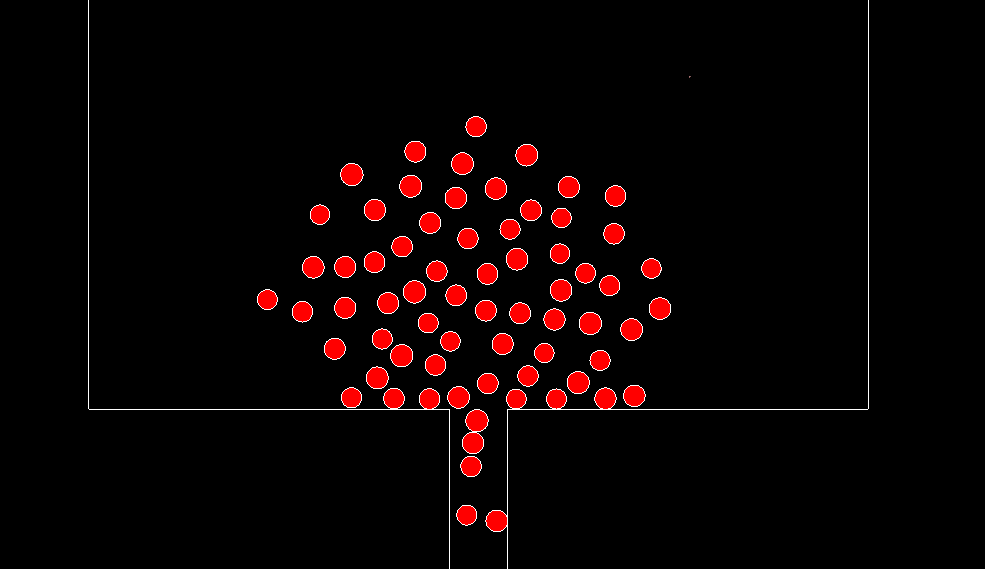
\includegraphics[width=6.5cm]{pics/program/room-no-future} 
        \par\end{centering}
        
        \caption{\label{fig:room-no-future} Room visualization}
    \end{figure}
    
    \begin{figure}[H]
        \centering{} 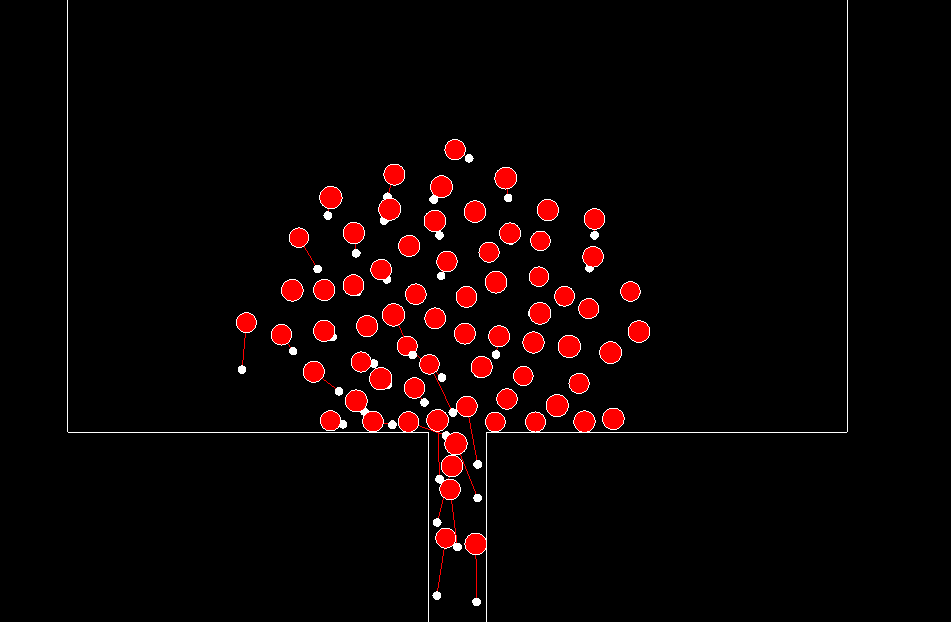
\includegraphics[width=6.5cm]{pics/program/room-future}
        \caption{\label{fig:room-future} Room visualization with visible future}
    \end{figure}
    
    The escape flow of pedestrians does not change drastically depending on the
    number of pedestrians, unlike the SFM. This happens because of the removal
    of the social force, which increased as pedestrians increased.

\section{Conclusion}
    
    Pedestrians can adjust their desired velocity at will, based on the
    data they perceive. We proposed a model that calculates the desired
    velocity of the social force model by conceptually moving the social
    force into the near future (FVP). The results look more natural than
    the original SFM and have been validated with experimental data. We
    used real-life metrics to validate our model, the results show that
    our model resembles reality with high fidelity. The proposed model
    produces a more natural navigation, but, at high densities, this isn't
    true, we still need further analysis of this scenario to adjust our
    model for both cases. \\
    In future work, the paths our virtual pedestrians
    may need to be compared and validated with real-life pedestrians
    paths to complement the use of metrics for the mean of pedestrians.
    Parameters should be re validated with more metrics and analyzed in
    even more detail. \\
    % It is important to notice that we have successfully removed the 
    % (undesired) social force from the original model and replacing it  
    % with the proposed changes, we were able reproduce real life results.
\newpage{}

\begin{thebibliography}{10}

\bibitem{key-hoog2004} Hoogendoorn, Serge P., and Piet HL Bovy. "Pedestrian route-choice and activity scheduling theory and models." Transportation Research Part B: Methodological 38.2 (2004): 169-190.

\bibitem{key-scha2009} Schadschneider, Andreas, et al. "Evacuation dynamics: Empirical results, modeling and applications." Encyclopedia of complexity and systems science. Springer New York, 2009. 3142-3176. 

\bibitem{key-scha2002} Schadschneider, Andreas. "Traffic flow: a statistical physics point of view." Physica A: Statistical Mechanics and its Applications 313.1 (2002): 153-187.

\bibitem{key-helb1995} Helbing, Dirk, and Peter Molnar. "Social force model for pedestrian dynamics." Physical review E 51.5 (1995): 4282.

\bibitem{key-helb2000} Helbing, Dirk, Illés Farkas, and Tamas Vicsek. "Simulating dynamical features of escape panic." Nature 407.6803 (2000): 487-490.

\bibitem{key-tara2005} Lakoba, Taras I., David J. Kaup, and Neal M. Finkelstein. "Modifications of the Helbing-Molnar-Farkas-Vicsek social force model for pedestrian evolution." Simulation 81.5 (2005): 339-352.

\bibitem{key-pari2009} Parisi, Daniel R., Marcelo Gilman, and Herman Moldovan. "A modification of the social force model can reproduce experimental data of pedestrian flows in normal conditions." Physica A: Statistical Mechanics and its Applications 388.17 (2009): 3600-3608.

\bibitem{key-kirc2002} Kirchner, Ansgar, and Andreas Schadschneider. "Simulation of evacuation processes using a bionics-inspired cellular automaton model for pedestrian dynamics." Physica A: Statistical Mechanics and its Applications 312.1 (2002): 260-276.

\bibitem{key-pari2011} Baglietto, Gabriel, and Daniel R. Parisi. "Continuous-space automaton model for pedestrian dynamics." Physical Review E 83.5 (2011): 056117.

\bibitem{key-kara2009} Karamouzas, Ioannis, et al. "A predictive collision avoidance model for pedestrian simulation." Motion in Games. Springer Berlin Heidelberg, 2009. 41-52.

\bibitem{key-kret2001} Kretz, Tobias, et al. "Quickest paths in simulations of pedestrians." Advances in Complex Systems 14.05 (2011): 733-759.

\bibitem{key-mous2009} Moussaïd, Mehdi, et al. "Experimental study of the behavioural mechanisms underlying self-organization in human crowds." Proceedings of the Royal Society B: Biological Sciences (2009): rspb-2009.

\bibitem{key-pedEvDyn2012} Weidmann, Ulrich, Uwe Kirsch, and Michael Schreckenberg, eds. Pedestrian and Evacuation Dynamics 2012. Springer Science \& Business, 2014.

\bibitem{key-qianLing2015} Qian-Ling, Wang, et al. "A new collision avoidance model for pedestrian dynamics." Chinese Physics B 24.3 (2015): 038901.

\end{thebibliography}

\end{document}
